% \documentclass[handout]{beamer}
\documentclass{beamer}

\mode<presentation>
{
  \usetheme{default}
  \usefonttheme[onlymath]{serif}
  % \usetheme{Singapore}
  % \usetheme{Warsaw}
  % \usetheme{Malmoe}
  % \useinnertheme{circles}
  % \useoutertheme{infolines}
  % \useinnertheme{rounded}

  \setbeamercovered{transparent=5}
}

\usepackage[english]{babel}
\usepackage[latin1]{inputenc}
\usepackage{alltt,listings,multirow,ulem,siunitx}
\usepackage[absolute,overlay]{textpos}
\TPGrid{1}{1}
\usepackage{pdfpages}
\usepackage{multimedia}
\usepackage{multicol}
\newcommand\hmmax{0}
\newcommand\bmmax{0}
\usepackage{bm}
\usepackage{comment}

% font definitions, try \usepackage{ae} instead of the following
% three lines if you don't like this look
\usepackage{mathptmx}
\usepackage[scaled=.90]{helvet}
% \usepackage{courier}
\usepackage[T1]{fontenc}
\usepackage{tikz}
\usetikzlibrary{decorations.pathreplacing}
\usetikzlibrary{shadows,arrows,shapes.misc,shapes.arrows,shapes.multipart,arrows,decorations.pathmorphing,backgrounds,positioning,fit,petri,calc,shadows,chains,matrix}


% \usepackage{pgfpages}
% \pgfpagesuselayout{4 on 1}[a4paper,landscape,border shrink=5mm]

\usepackage{JedMacros}

\newcommand{\timeR}{t_{\mathrm{R}}}
\newcommand{\timeW}{t_{\mathrm{W}}}
\newcommand{\mglevel}{\ensuremath{\ell}}
\newcommand{\mglevelcp}{\ensuremath{\mglevel_{\mathrm{cp}}}}
\newcommand{\mglevelcoarse}{\ensuremath{\mglevel_{\mathrm{coarse}}}}
\newcommand{\mglevelfine}{\ensuremath{\mglevel_{\mathrm{fine}}}}

%solution and residual
\newcommand{\vx}{\ensuremath{x}}
\newcommand{\vc}{\ensuremath{\hat{x}}}
\newcommand{\vr}{\ensuremath{r}}
\newcommand{\vb}{\ensuremath{b}}

%operators
\newcommand{\vA}{\ensuremath{A}}
\newcommand{\vP}{\ensuremath{I_H^h}}
\newcommand{\vS}{\ensuremath{S}}
\newcommand{\vR}{\ensuremath{I_h^H}}
\newcommand{\vI}{\ensuremath{\hat I_h^H}}
\newcommand{\vV}{\ensuremath{\mathbf{V}}}
\newcommand{\vF}{\ensuremath{F}}
\newcommand{\vtau}{\ensuremath{\mathbf{\tau}}}


\title{Sharing Thread Pools and Caches for Inter-library Composition and Multicore Performance}
\author{{\bf Jed Brown}, Shrirang Abhyankar, Barry Smith}

% - Use the \inst command only if there are several affiliations.
% - Keep it simple, no one is interested in your street address.
\institute
{
  Mathematics and Computer Science Division, Argonne National Laboratory
}

\date{SIAM CSE, 2013-02-28}

% This is only inserted into the PDF information catalog. Can be left
% out.
\subject{Talks}


% If you have a file called "university-logo-filename.xxx", where xxx
% is a graphic format that can be processed by latex or pdflatex,
% resp., then you can add a logo as follows:

% \pgfdeclareimage[height=0.5cm]{university-logo}{university-logo-filename}
% \logo{\pgfuseimage{university-logo}}



% Delete this, if you do not want the table of contents to pop up at
% the beginning of each subsection:
% \AtBeginSubsection[]
% {
% \begin{frame}<beamer>
%   \frametitle{Outline}
%   \tableofcontents[currentsection,currentsubsection]
% \end{frame}
% }

\AtBeginSection[]
{
  \begin{frame}<beamer>
    \frametitle{Outline}
    \tableofcontents[currentsection]
  \end{frame}
}

% If you wish to uncover everything in a step-wise fashion, uncomment
% the following command:

% \beamerdefaultoverlayspecification{<+->}

\begin{document}
\lstset{language=C}
\normalem

\begin{frame}
  \titlepage
\end{frame}

\begin{frame}
  \begin{itemize} \Large
  \item Parallel computing used to be about computing.
  \item<2> \alert{It's increasingly about data movement.}
  \end{itemize}
\end{frame}

\begin{frame}{Libraries and threads}
  \begin{itemize}
  \item Purpose of threads
    \begin{itemize}
    \item Reduce memory usage for executable code and shared/global data structures
    \item Reduce resource contention (network, filesystem)
    \item Encourage cache and bandwidth sharing
    \end{itemize}
  \item Different ways to use threads
    \begin{itemize}
    \item Large dense linear algebra: use theads internally. User only interacts with serial interface.
    \item OMP parallel at \texttt{main} and shared nothing by default.
    \item \texttt{MPI\_Comm\_split\_type()} and \texttt{MPI\_Win\_allocate\_shared()}
    \end{itemize}
  \item Competing standards: OpenMP, TBB, Pthreads, OpenCL, \ldots
    \begin{itemize}
    \item Targeted at applications, not libraries
    \item Poor support for sharing
    \end{itemize}
  \item Unfriendly to require \texttt{MPI\_THREAD\_MULTIPLE}
  \end{itemize}
\end{frame}

\begin{frame}{Maintaining libraries}
  \begin{itemize}
  \item PETSc developers receive about 100 user messages per day
    \begin{itemize}
    \item Configuration/installation (with broken environment)
    \item API (mis)usage
    \item Understanding performance/variability
    \item Solver convergence, selection of methods, and 
    \end{itemize}
  \item $>10\%$ of PETSc is pure input validation and debuggability
    \begin{itemize}
    \item Diagnose bugs in user code over email from our error messages
    \item Valgrind-like memory tracing and sentinels, explicit stack for signal handlers, pointer testing
    \item Compiled out in optimized builds
    \end{itemize}
  \item $3\%$ of PETSc is profiling/performance diagnostics
  \item Memory-related performance problems are \alert<2>{difficult to debug}
  \item Thread placement and affinity is \alert<3>{fragile}
  \end{itemize}
\end{frame}

\begin{frame}{Virtual addressing and ``first touch''}
  \begin{itemize}
  \item Virtual memory is unavoidable for NUMA with shared memory programming.
    \begin{itemize}
    \item Can speculate that Blue Gene/Q is UMA \emph{because} of TLB allergies (preference for offset-mapped shared memory)
    \end{itemize}
  \item Most systems with virtual memory do not find physical pages when you call \texttt{malloc()}.
  \item The kernel finds physical pages when you trigger a page fault, usually ``close to'' the thread causing the page fault.
  \item \texttt{
      cache and TLB information (2): \\
      \quad 0x5a: data TLB: 2M/4M pages, 4-way, 32 entries \\
      \quad 0x03: data TLB: 4K pages, 4-way, 64 entries}
  \item Inspecting or changing location of physical pages is not portable (\texttt{hwloc} does the best they can).
  \item<2> \alert{Implicitness} is bad for libraries and bad for support
  \end{itemize}
\end{frame}

\begin{frame}{What can go wrong?}
  \begin{columns}
    \begin{column}{0.4\textwidth}
      \begin{itemize} \small
      \item Memory performance depends on socket connectivity
      \item Unbalanced prior allocations
      \item Cache coherence costs (e.g., STREAM at 50\% of bus bandwidth)
      \item Thread can migrate away
      \item Linux-2.6.38 has transparent huge pages (2M/4M versus 4K)
      \item \texttt{libhugetlbfs} not widely installed
      \end{itemize}
    \end{column}
    \begin{column}{0.6\textwidth}
      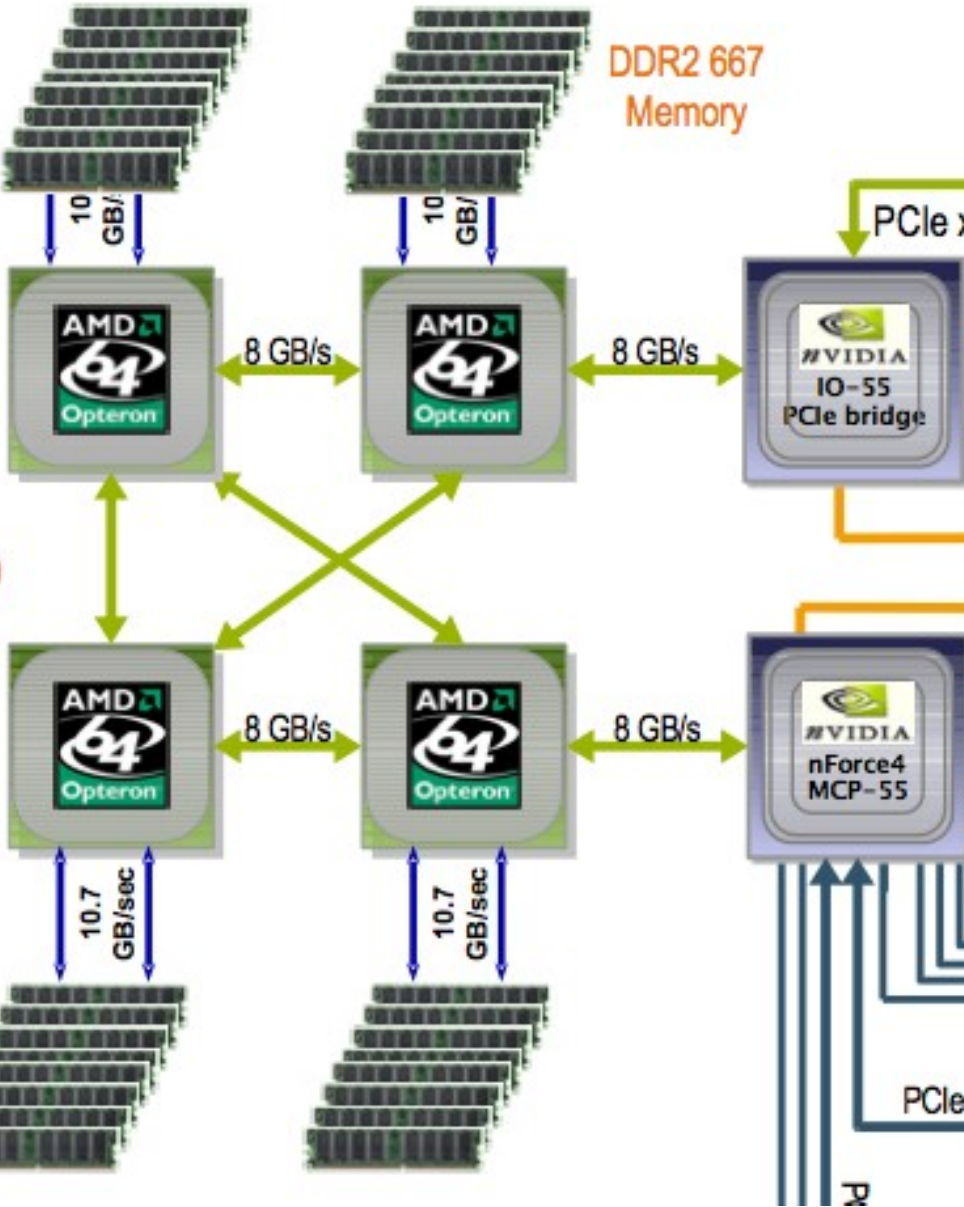
\includegraphics[width=\textwidth]{figures/hardware/AMDMemory}
    \end{column}
  \end{columns}
\end{frame}

\begin{frame}{With all these problems, why use common allocation?}
  \begin{itemize}
  \item Data structures are simpler, smaller, and share more easily.
    \begin{itemize}
    \item Consider sparse matrix-matrix multiply
    \end{itemize}
  \item Cache/bandwidth sharing are key reasons for threads in the first place
  \item Compatibility with user expectation
  \item Ability to mix optimized threaded code with legacy unthreaded
  \item Separate allocation is sometimes feasible and can work very well
  \end{itemize}
\end{frame}

\begin{frame}{Speed of light and cost of synchronization}
  \begin{itemize}
  \item Fundamental lower bound: several clock cycles for light to make round trip across an Ivy Bridge die
  \item 
    \begin{tabular}{lrr}
      \toprule
      Operation (16-CPU X5550 Nehalem) & Time (ns) & Clocks \\
      \midrule
      Clock period (two packed FP instructions) & 0.4 & 1 \\
      Best case CAS & 12.2 & 33.8 \\
      Best-case lock/unlock & 25.6 & 71.2 \\
      Single cache miss & 12.9 & 35.8 \\
      CAS cache miss & 7.0 & 19.4 \\
      Single cache-miss {\bf(off-core)} & 31.2 & 86.6 \\
      CAS cache miss {\bf (off-core)} & 31.2 & 86.5 \\
      Single cache miss {\bf (off-socket)} & 92.4 & 256.7 \\
      CAS cache miss {\bf (off-socket)} & 95.9 & 266.4 \\
      \bottomrule
    \end{tabular}
  \item From Paul McKenney, see \url{http://www.rdrop.com/users/paulmck/RCU/}
  \end{itemize}
\end{frame}

\begin{frame}{Synchronization mechanisms}
  \begin{itemize}
  \item OpenMP over-synchronizes by default
  \item OMP \texttt{nowait} clause is global and of limited utility
  \item OMP \texttt{critical} is fundamentally not scalable
  \item OMP \texttt{atomic} cause excessive cache-line bouncing
  \item Collectives like \texttt{allreduce} and \texttt{scan} can be scalable
  \item Mechanisms like RCU (Read-Copy Update) allow safe, mostly-unstructured asynchronous shared mutable state
  \item TBB synchronization is either non-scalable (e.g., mutexes) or tighly coupled to tasks
  \end{itemize}
\end{frame}

\begin{frame}{Will Transactional Memory save the day?}
  \begin{itemize}
  \item TM is good for large scattered writes over data structures that cannot be partitioned.
  \item TM is expensive relative to locks for small writes
  \item Implementations and performance is highly variable
  \item Non-idempotent operations may be applied multiple times on retry
  \item McKenney, Michael, Triplett, Walpole (2010) ``Why the grass may not be greener on the other side: A comparison of locking versus transactional memory''.
  \end{itemize}
\end{frame}

\begin{frame}{PETSc: ``E'' is for \emph{Extensible}}
  \begin{itemize}
  \item Ideal: anything that can be developed in the library can also be developed as a plugin.
    \begin{itemize}
    \item Matrix and vector formats
    \item Preconditioners
    \item Krylov methods
    \end{itemize}
  \item High-level plugins do not want to think about threads
  \item Low-level plugins need low-level access
  \item Ability to call internal functions \emph{from threads}
  \end{itemize}
\end{frame}

\begin{frame}{Thread Communicator design goals}
  \begin{itemize}
  \item Run-time choice of common threading environments
  \item Ability to split communicators
  \item Non-blocking job submission of collective jobs (perhaps on subcomms)
  \item Thread collectives like reductions and scans decoupled from tasks
  \item Collective asynchronous and synchronous jobs
  \item Avoid over-synchronization: hazard pointers, RCU (unfortunately a patent minefield for non-LGPL)
  \item Library isolation, attribute caching
  \end{itemize}
\end{frame}

\begin{frame}[fragile]{\texttt{PetscThreadComm}}
  \begin{itemize}
  \item Attached to \texttt{MPI\_Comm} which is used in existing interfaces
  \item Split and dup based on topology
    \begin{itemize}
    \item runs asynchronously if thread rank 0 is not in comm
    \end{itemize}
  \item Asynchronous reductions: {\scriptsize
    \begin{minted}{c}
    void VecDot_k(int thread_id,Vec X,Vec Y,PetscThreadReduction red) {
      int rstart,rend;
      const Scalar *x,*y;
      VecGetThreadOwnershipRange(X,thread_id,&rstart,&rend);
      VecGetArrayRead(X,&x);
      VecGetArrayRead(Y,&y);
      Scalar a = BLASdot_(x[rstart:rstart+rend],y[rstart:rstart+rend]);
      PetscThreadReductionPost_k(thread_id,red,&a);
    }
    void VecDot(Vec X,Vec Y,Scalar *a) {
      ...
      PetscCommRunKernel3(X->comm,VecDot_k,X,Y,red);
      PetscThreadReductionEnd(red,a); // or PetscThreadReductionEnd_k()
    }
    \end{minted}
    }
  \item Can also call \cfunc|VecDot_k| from another kernel
  \end{itemize}
\end{frame}

\begin{frame}{Expressing memory layout}
  \begin{itemize}
  \item PETSc vectors and matrices have \texttt{PetscLayout}
  \item Provides sufficient local view of distribution across distributed memory
  \item Now includes thread ownership ranges
  \item Implementations can extend to richer descriptions
    \begin{itemize}
    \item Grouping and interlacing
    \end{itemize}
  \end{itemize}
\end{frame}

\begin{frame}{Hardware Arithmetic Intensity}
  \begin{tabular}{lc}
    \toprule
    Operation                         & Arithmetic Intensity (flops per byte) \\
    \midrule
    Sparse matrix-vector product      & 1/6                  \\
    Dense matrix-vector product       & 1/4                  \\
    Unassembled matrix-vector product & $\approx 8$          \\
    High-order residual evaluation    & $> 5$                \\
    \bottomrule
  \end{tabular}
  \bigskip
  \begin{tabular}{lrrr}
    \toprule
    Processor           & BW (GB/s) & Peak (GF/s) & Balanced AI (F/B) \\
    \midrule
    Sandy Bridge 6-core & 21*       & 150         & 7.2                 \\
    Magny Cours 16-core & 42*       & 281         & 6.7                 \\
    Blue Gene/Q node    & 43        & 205         & 4.8                 \\
    GeForce 9400M       & 21        & 54          & 2.6                 \\
    GTX 285             & 159       & 1062        & 6.8                 \\
    Tesla M2050         & 144       & 1030        & 7.1                 \\
    \bottomrule
  \end{tabular}
\end{frame}

\begin{frame}[shrink=5]{Performance of assembled versus unassembled}
  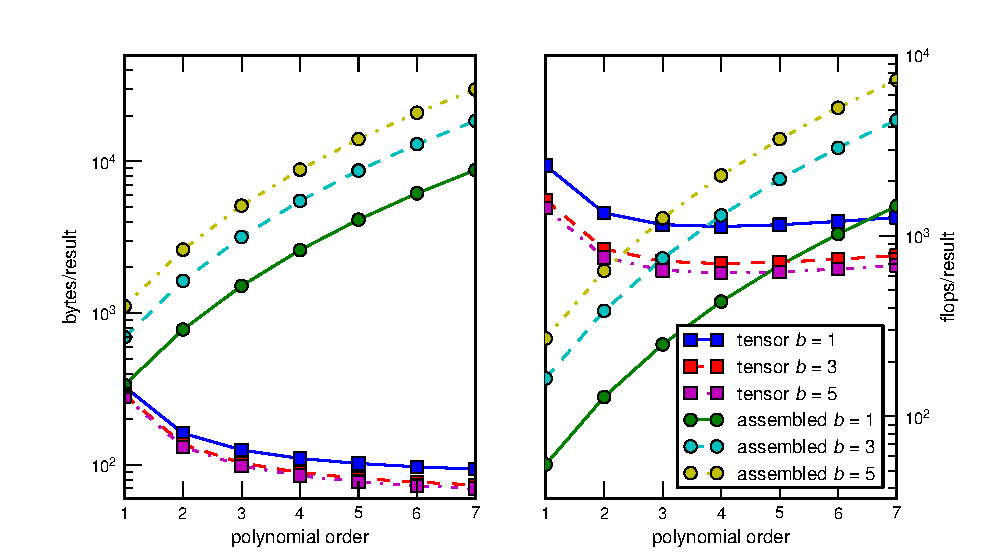
\includegraphics[width=\textwidth]{figures/TensorVsAssembly} \\
  \begin{itemize}
  \item High order Jacobian stored unassembled using coefficients at quadrature points, can use local AD
  \item Choose approximation order at run-time, independent for each field
  \item Precondition high order using assembled lowest order method
  \item Implementation $> 70\%$ of FPU peak, SpMV bandwidth wall $< 4\%$
  \end{itemize}
\end{frame}


\begin{frame}{Reducing memory bandwidth}
  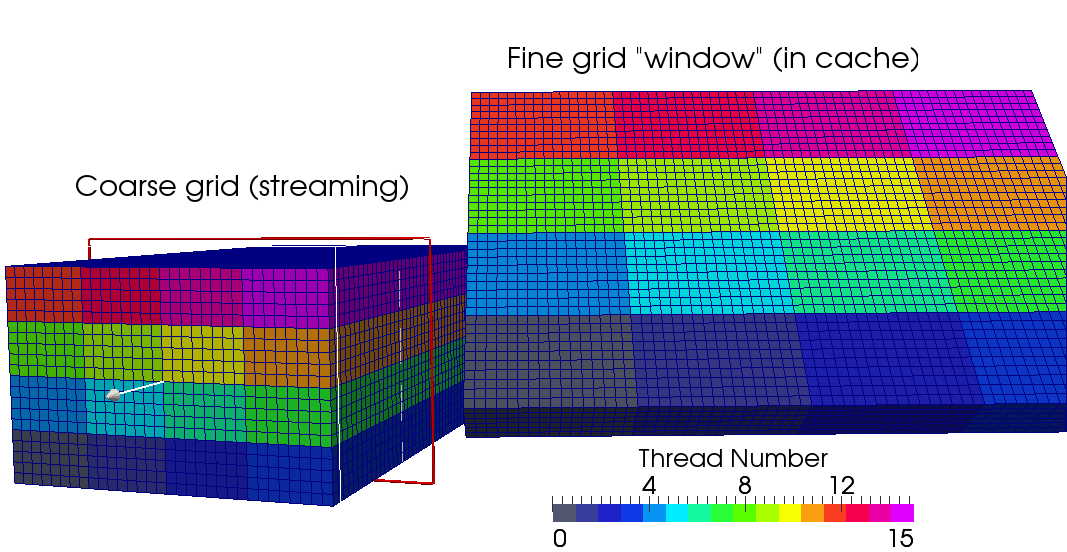
\includegraphics[width=\textwidth]{figures/MG/SRMGWindow}
  \begin{itemize}
  \item Sweep through ``coarse'' grid with moving window
  \item Zoom in on new slab, construct fine grid ``window'' in-cache
  \item Interpolate to new fine grid, apply pipelined smoother ($s$-step)
  \item Compute residual, accumulate restriction of state and residual into coarse grid, expire slab from window
  \end{itemize}
\end{frame}

\begin{frame}{Arithmetic intensity of sweeping visit}
  \begin{itemize}
  \item Assume 3D cell-centered, 7-point stencil
  \item 14 flops/cell for second order interpolation
  \item $\ge 15$ flops/cell for fine-grid residual or point smoother
  \item 2 flops/cell to enforce coarse-grid compatibility
  \item 2 flops/cell for plane restriction
  \item assume coarse grid points are reused in cache
  \item Fused visit reads $u^H$ and writes $\hat I_h^H u^h$ and $I_h^H r^h$
  \item Arithmetic Intensity
    \begin{equation}
      \frac{{\overbrace{15}^{\text{interp}}} + {\overbrace{2\cdot (15+2)}^{\text{compatible relaxation}}} + \overbrace{2\cdot 15}^{\text{smooth}} + \overbrace{15}^{\text{residual}} + \overbrace{2}^{\text{restrict}}}{3 \cdot \texttt{sizeof(scalar)} / \underbrace{2^3}_{\text{coarsening}}} \gtrsim 30
    \end{equation}
  \item Still $\gtrsim 10$ with non-compressible fine-grid forcing
  \end{itemize}
\end{frame}

\begin{frame}{Outlook}
  \begin{itemize}
  \item \texttt{PetscThreadComm} with pthreads lower overhead than OpenMP
    \begin{itemize}
    \item Weaker synchronization, fewer memory fences
    \end{itemize}
  \item Enable better reuse of ``kernels''
  \item Thread organization more explicit, can cross library boundaries
  \item Performance and correctness debuggability via email/error messages
  \item Allow transition from calling via outer interfaces to calling from threads
  \item Matrix-free methods reduce bandwidth requirements
    \begin{itemize}
    \item can simplify memory management, but the user is no longer isolated from solvers
    \end{itemize}
  \item Exotic algorithms can move us back to FPU-limited
    \begin{itemize}
    \item Don't have to worry so much about memory
    \item Such algorithms are often cache-intensive so need to share
    \end{itemize}
  \item Portable Hardware Locality \url{http://open-mpi.org/projects/hwloc}
  \item Concurrency Kit \url{http://concurrencykit.org}
  \end{itemize}
\end{frame}

\end{document}
